% 债券期货计算图 (Hull Example 6-2) - 可在一级模考卷.tex 中 % 债券期货计算图 (Hull Example 6-2) - 可在一级模考卷.tex 中 % 债券期货计算图 (Hull Example 6-2) - 可在一级模考卷.tex 中 % 债券期货计算图 (Hull Example 6-2) - 可在一级模考卷.tex 中 \input{bond-futures-figure}
% 需在导言区已有: \usepackage{xcolor}, \usepackage{tikz}, \newcommand{\dollar}{...}

\noindent
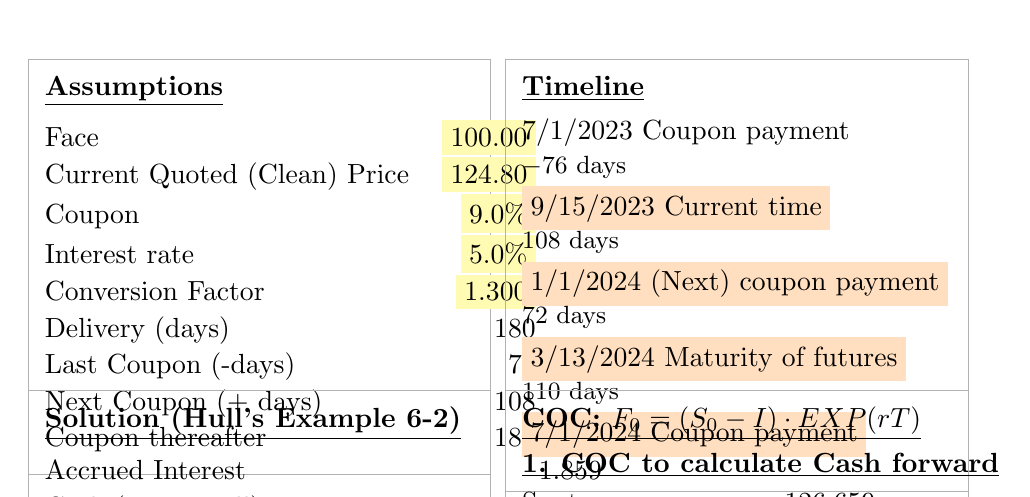
\begin{tikzpicture}[
  box/.style={draw=gray!60, line width=0.4pt, inner sep=6pt, minimum width=0.45\textwidth, minimum height=0pt, align=flush left, anchor=north west},
]
  \useasboundingbox (0,-5.2) rectangle (1.02\textwidth, 0.4);
  \node[box] (A) at (0,0) {
    \begin{minipage}[t]{0.44\textwidth}
      \textbf{\underline{Assumptions}}\\[4pt]
      \renewcommand{\arraystretch}{1.1}
      \begin{tabular}{@{}lr@{}}
        Face & \colorbox{yellow!30}{\dollar100.00} \\
        Current Quoted (Clean) Price & \colorbox{yellow!30}{\dollar124.80} \\
        Coupon & \colorbox{yellow!30}{9.0\%} \\
        Interest rate & \colorbox{yellow!30}{5.0\%} \\
        Conversion Factor & \colorbox{yellow!30}{1.300} \\
        Delivery (days) & 180 \\
        Last Coupon (-days) & 76 \\
        Next Coupon (+ days) & 108 \\
        Coupon thereafter & 182 \\
      \end{tabular}
    \end{minipage}
  };
  \node[box] (B) at (0.5\textwidth,0) {
    \begin{minipage}[t]{0.44\textwidth}
      \textbf{\underline{Timeline}}\\[4pt]
      7/1/2023 Coupon payment\\
      \hfill {\small $-76$ days}\\[2pt]
      \colorbox{orange!25}{9/15/2023 Current time}\\
      \hfill {\small 108 days}\\[2pt]
      \colorbox{orange!25}{1/1/2024 (Next) coupon payment}\\
      \hfill {\small 72 days}\\[2pt]
      \colorbox{orange!25}{3/13/2024 Maturity of futures}\\
      \hfill {\small 110 days}\\[2pt]
      \colorbox{orange!25}{7/1/2024 Coupon payment}\\
    \end{minipage}
  };

  \node[box] (C) at (0,-4.2) {
    \begin{minipage}[t]{0.44\textwidth}
      \textbf{\underline{Solution (Hull's Example 6-2)}}\\[4pt]
      \begin{tabular}{@{}lr@{}}
        Accrued Interest & \dollar1.859 \\
        Cash (Dirty, Full) Price & \dollar126.6587 \\
        PV of next coupon & \colorbox{yellow!30}{\dollar4.434} \\
        Cash Futures Price & \colorbox{yellow!30}{\dollar125.2760} \\
        Days Accrued @ delivery & 72 \\
        Days Remain @ delivery & 110 \\
        Futures price, Quoted, 12\% bond & \dollar123.4958 \\
        Futures price, Quoted, CTD & \colorbox{yellow!30}{\dollar94.9968} \\
      \end{tabular}
    \end{minipage}
  };
  \node[box] (D) at (0.5\textwidth,-4.2) {
    \begin{minipage}[t]{0.44\textwidth}
      \textbf{\underline{COC: $F_0=(S_0-I)\cdot\text{EXP}(rT)$}}\\[4pt]
      \textbf{\underline{1. COC to calculate Cash forward}}\\[2pt]
      \begin{tabular}{@{}lr@{}}
        Spot & \dollar126.659 \\
        Income & \dollar4.434 \\
        Forward cash price & \underline{\dollar125.276} \\
      \end{tabular}\\[6pt]
      \textbf{\underline{2. Then dirty --> clean \& standardize}}\\[2pt]
      \begin{tabular}{@{}lr@{}}
        Subtract AI & \dollar1.780 \\
        Quoted Price, 12\% bond = & \dollar123.496 \\
        Divide by CF of 1.30: & \dollar94.997 \\
      \end{tabular}
    \end{minipage}
  };
\end{tikzpicture}

% 需在导言区已有: \usepackage{xcolor}, \usepackage{tikz}, \newcommand{\dollar}{...}

\noindent
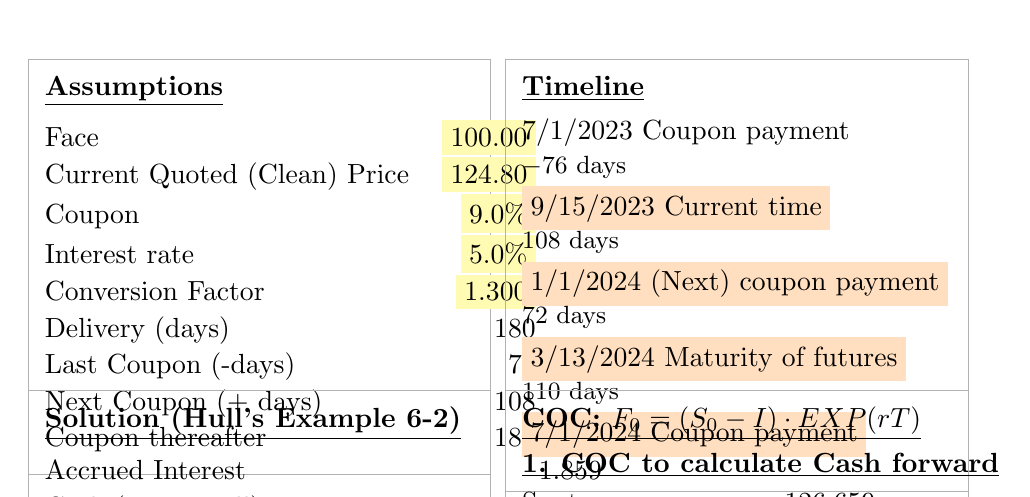
\begin{tikzpicture}[
  box/.style={draw=gray!60, line width=0.4pt, inner sep=6pt, minimum width=0.45\textwidth, minimum height=0pt, align=flush left, anchor=north west},
]
  \useasboundingbox (0,-5.2) rectangle (1.02\textwidth, 0.4);
  \node[box] (A) at (0,0) {
    \begin{minipage}[t]{0.44\textwidth}
      \textbf{\underline{Assumptions}}\\[4pt]
      \renewcommand{\arraystretch}{1.1}
      \begin{tabular}{@{}lr@{}}
        Face & \colorbox{yellow!30}{\dollar100.00} \\
        Current Quoted (Clean) Price & \colorbox{yellow!30}{\dollar124.80} \\
        Coupon & \colorbox{yellow!30}{9.0\%} \\
        Interest rate & \colorbox{yellow!30}{5.0\%} \\
        Conversion Factor & \colorbox{yellow!30}{1.300} \\
        Delivery (days) & 180 \\
        Last Coupon (-days) & 76 \\
        Next Coupon (+ days) & 108 \\
        Coupon thereafter & 182 \\
      \end{tabular}
    \end{minipage}
  };
  \node[box] (B) at (0.5\textwidth,0) {
    \begin{minipage}[t]{0.44\textwidth}
      \textbf{\underline{Timeline}}\\[4pt]
      7/1/2023 Coupon payment\\
      \hfill {\small $-76$ days}\\[2pt]
      \colorbox{orange!25}{9/15/2023 Current time}\\
      \hfill {\small 108 days}\\[2pt]
      \colorbox{orange!25}{1/1/2024 (Next) coupon payment}\\
      \hfill {\small 72 days}\\[2pt]
      \colorbox{orange!25}{3/13/2024 Maturity of futures}\\
      \hfill {\small 110 days}\\[2pt]
      \colorbox{orange!25}{7/1/2024 Coupon payment}\\
    \end{minipage}
  };

  \node[box] (C) at (0,-4.2) {
    \begin{minipage}[t]{0.44\textwidth}
      \textbf{\underline{Solution (Hull's Example 6-2)}}\\[4pt]
      \begin{tabular}{@{}lr@{}}
        Accrued Interest & \dollar1.859 \\
        Cash (Dirty, Full) Price & \dollar126.6587 \\
        PV of next coupon & \colorbox{yellow!30}{\dollar4.434} \\
        Cash Futures Price & \colorbox{yellow!30}{\dollar125.2760} \\
        Days Accrued @ delivery & 72 \\
        Days Remain @ delivery & 110 \\
        Futures price, Quoted, 12\% bond & \dollar123.4958 \\
        Futures price, Quoted, CTD & \colorbox{yellow!30}{\dollar94.9968} \\
      \end{tabular}
    \end{minipage}
  };
  \node[box] (D) at (0.5\textwidth,-4.2) {
    \begin{minipage}[t]{0.44\textwidth}
      \textbf{\underline{COC: $F_0=(S_0-I)\cdot\text{EXP}(rT)$}}\\[4pt]
      \textbf{\underline{1. COC to calculate Cash forward}}\\[2pt]
      \begin{tabular}{@{}lr@{}}
        Spot & \dollar126.659 \\
        Income & \dollar4.434 \\
        Forward cash price & \underline{\dollar125.276} \\
      \end{tabular}\\[6pt]
      \textbf{\underline{2. Then dirty --> clean \& standardize}}\\[2pt]
      \begin{tabular}{@{}lr@{}}
        Subtract AI & \dollar1.780 \\
        Quoted Price, 12\% bond = & \dollar123.496 \\
        Divide by CF of 1.30: & \dollar94.997 \\
      \end{tabular}
    \end{minipage}
  };
\end{tikzpicture}

% 需在导言区已有: \usepackage{xcolor}, \usepackage{tikz}, \newcommand{\dollar}{...}

\noindent
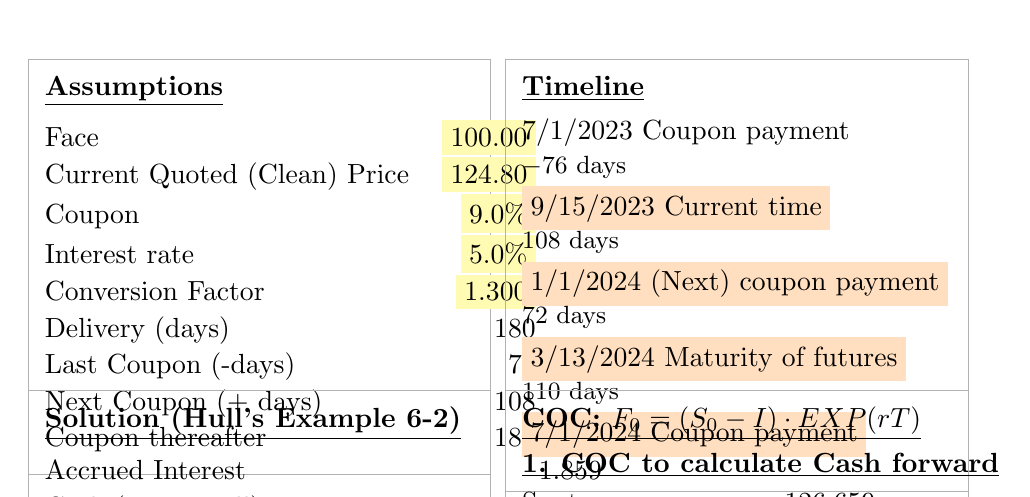
\begin{tikzpicture}[
  box/.style={draw=gray!60, line width=0.4pt, inner sep=6pt, minimum width=0.45\textwidth, minimum height=0pt, align=flush left, anchor=north west},
]
  \useasboundingbox (0,-5.2) rectangle (1.02\textwidth, 0.4);
  \node[box] (A) at (0,0) {
    \begin{minipage}[t]{0.44\textwidth}
      \textbf{\underline{Assumptions}}\\[4pt]
      \renewcommand{\arraystretch}{1.1}
      \begin{tabular}{@{}lr@{}}
        Face & \colorbox{yellow!30}{\dollar100.00} \\
        Current Quoted (Clean) Price & \colorbox{yellow!30}{\dollar124.80} \\
        Coupon & \colorbox{yellow!30}{9.0\%} \\
        Interest rate & \colorbox{yellow!30}{5.0\%} \\
        Conversion Factor & \colorbox{yellow!30}{1.300} \\
        Delivery (days) & 180 \\
        Last Coupon (-days) & 76 \\
        Next Coupon (+ days) & 108 \\
        Coupon thereafter & 182 \\
      \end{tabular}
    \end{minipage}
  };
  \node[box] (B) at (0.5\textwidth,0) {
    \begin{minipage}[t]{0.44\textwidth}
      \textbf{\underline{Timeline}}\\[4pt]
      7/1/2023 Coupon payment\\
      \hfill {\small $-76$ days}\\[2pt]
      \colorbox{orange!25}{9/15/2023 Current time}\\
      \hfill {\small 108 days}\\[2pt]
      \colorbox{orange!25}{1/1/2024 (Next) coupon payment}\\
      \hfill {\small 72 days}\\[2pt]
      \colorbox{orange!25}{3/13/2024 Maturity of futures}\\
      \hfill {\small 110 days}\\[2pt]
      \colorbox{orange!25}{7/1/2024 Coupon payment}\\
    \end{minipage}
  };

  \node[box] (C) at (0,-4.2) {
    \begin{minipage}[t]{0.44\textwidth}
      \textbf{\underline{Solution (Hull's Example 6-2)}}\\[4pt]
      \begin{tabular}{@{}lr@{}}
        Accrued Interest & \dollar1.859 \\
        Cash (Dirty, Full) Price & \dollar126.6587 \\
        PV of next coupon & \colorbox{yellow!30}{\dollar4.434} \\
        Cash Futures Price & \colorbox{yellow!30}{\dollar125.2760} \\
        Days Accrued @ delivery & 72 \\
        Days Remain @ delivery & 110 \\
        Futures price, Quoted, 12\% bond & \dollar123.4958 \\
        Futures price, Quoted, CTD & \colorbox{yellow!30}{\dollar94.9968} \\
      \end{tabular}
    \end{minipage}
  };
  \node[box] (D) at (0.5\textwidth,-4.2) {
    \begin{minipage}[t]{0.44\textwidth}
      \textbf{\underline{COC: $F_0=(S_0-I)\cdot\text{EXP}(rT)$}}\\[4pt]
      \textbf{\underline{1. COC to calculate Cash forward}}\\[2pt]
      \begin{tabular}{@{}lr@{}}
        Spot & \dollar126.659 \\
        Income & \dollar4.434 \\
        Forward cash price & \underline{\dollar125.276} \\
      \end{tabular}\\[6pt]
      \textbf{\underline{2. Then dirty --> clean \& standardize}}\\[2pt]
      \begin{tabular}{@{}lr@{}}
        Subtract AI & \dollar1.780 \\
        Quoted Price, 12\% bond = & \dollar123.496 \\
        Divide by CF of 1.30: & \dollar94.997 \\
      \end{tabular}
    \end{minipage}
  };
\end{tikzpicture}

% 需在导言区已有: \usepackage{xcolor}, \usepackage{tikz}, \newcommand{\dollar}{...}

\noindent
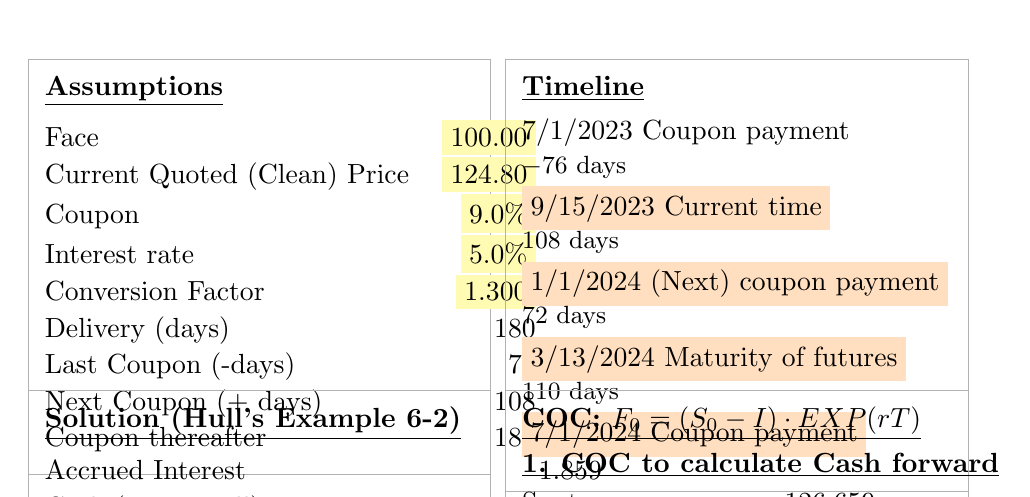
\begin{tikzpicture}[
  box/.style={draw=gray!60, line width=0.4pt, inner sep=6pt, minimum width=0.45\textwidth, minimum height=0pt, align=flush left, anchor=north west},
]
  \useasboundingbox (0,-5.2) rectangle (1.02\textwidth, 0.4);
  \node[box] (A) at (0,0) {
    \begin{minipage}[t]{0.44\textwidth}
      \textbf{\underline{Assumptions}}\\[4pt]
      \renewcommand{\arraystretch}{1.1}
      \begin{tabular}{@{}lr@{}}
        Face & \colorbox{yellow!30}{\dollar100.00} \\
        Current Quoted (Clean) Price & \colorbox{yellow!30}{\dollar124.80} \\
        Coupon & \colorbox{yellow!30}{9.0\%} \\
        Interest rate & \colorbox{yellow!30}{5.0\%} \\
        Conversion Factor & \colorbox{yellow!30}{1.300} \\
        Delivery (days) & 180 \\
        Last Coupon (-days) & 76 \\
        Next Coupon (+ days) & 108 \\
        Coupon thereafter & 182 \\
      \end{tabular}
    \end{minipage}
  };
  \node[box] (B) at (0.5\textwidth,0) {
    \begin{minipage}[t]{0.44\textwidth}
      \textbf{\underline{Timeline}}\\[4pt]
      7/1/2023 Coupon payment\\
      \hfill {\small $-76$ days}\\[2pt]
      \colorbox{orange!25}{9/15/2023 Current time}\\
      \hfill {\small 108 days}\\[2pt]
      \colorbox{orange!25}{1/1/2024 (Next) coupon payment}\\
      \hfill {\small 72 days}\\[2pt]
      \colorbox{orange!25}{3/13/2024 Maturity of futures}\\
      \hfill {\small 110 days}\\[2pt]
      \colorbox{orange!25}{7/1/2024 Coupon payment}\\
    \end{minipage}
  };

  \node[box] (C) at (0,-4.2) {
    \begin{minipage}[t]{0.44\textwidth}
      \textbf{\underline{Solution (Hull's Example 6-2)}}\\[4pt]
      \begin{tabular}{@{}lr@{}}
        Accrued Interest & \dollar1.859 \\
        Cash (Dirty, Full) Price & \dollar126.6587 \\
        PV of next coupon & \colorbox{yellow!30}{\dollar4.434} \\
        Cash Futures Price & \colorbox{yellow!30}{\dollar125.2760} \\
        Days Accrued @ delivery & 72 \\
        Days Remain @ delivery & 110 \\
        Futures price, Quoted, 12\% bond & \dollar123.4958 \\
        Futures price, Quoted, CTD & \colorbox{yellow!30}{\dollar94.9968} \\
      \end{tabular}
    \end{minipage}
  };
  \node[box] (D) at (0.5\textwidth,-4.2) {
    \begin{minipage}[t]{0.44\textwidth}
      \textbf{\underline{COC: $F_0=(S_0-I)\cdot\text{EXP}(rT)$}}\\[4pt]
      \textbf{\underline{1. COC to calculate Cash forward}}\\[2pt]
      \begin{tabular}{@{}lr@{}}
        Spot & \dollar126.659 \\
        Income & \dollar4.434 \\
        Forward cash price & \underline{\dollar125.276} \\
      \end{tabular}\\[6pt]
      \textbf{\underline{2. Then dirty --> clean \& standardize}}\\[2pt]
      \begin{tabular}{@{}lr@{}}
        Subtract AI & \dollar1.780 \\
        Quoted Price, 12\% bond = & \dollar123.496 \\
        Divide by CF of 1.30: & \dollar94.997 \\
      \end{tabular}
    \end{minipage}
  };
\end{tikzpicture}
